\section{Dataset Processing}

In this project, we apply methods to the UT Zappos50K dataset \cite{yu2014fine}, which is a large shoe dataset. It collected more than 50,000 images of shoes from Zappos.com \cite{}. The dataset contains four main classes, which are shoes, sandals, slippers, and boots. Each category is a sub-folder under the root directory. In each category folder, the images are divided into several sub-folders based on the functional types, followed by the individual brands. Figure \ref{fig:data_folder} shows an example of the structure of the dataset. Figure \ref{fig:data_example} illustrates the five samples in the four categories. We can observe that each image is centered on a white background and pictured in the same orientation. 

\begin{figure}[h]
	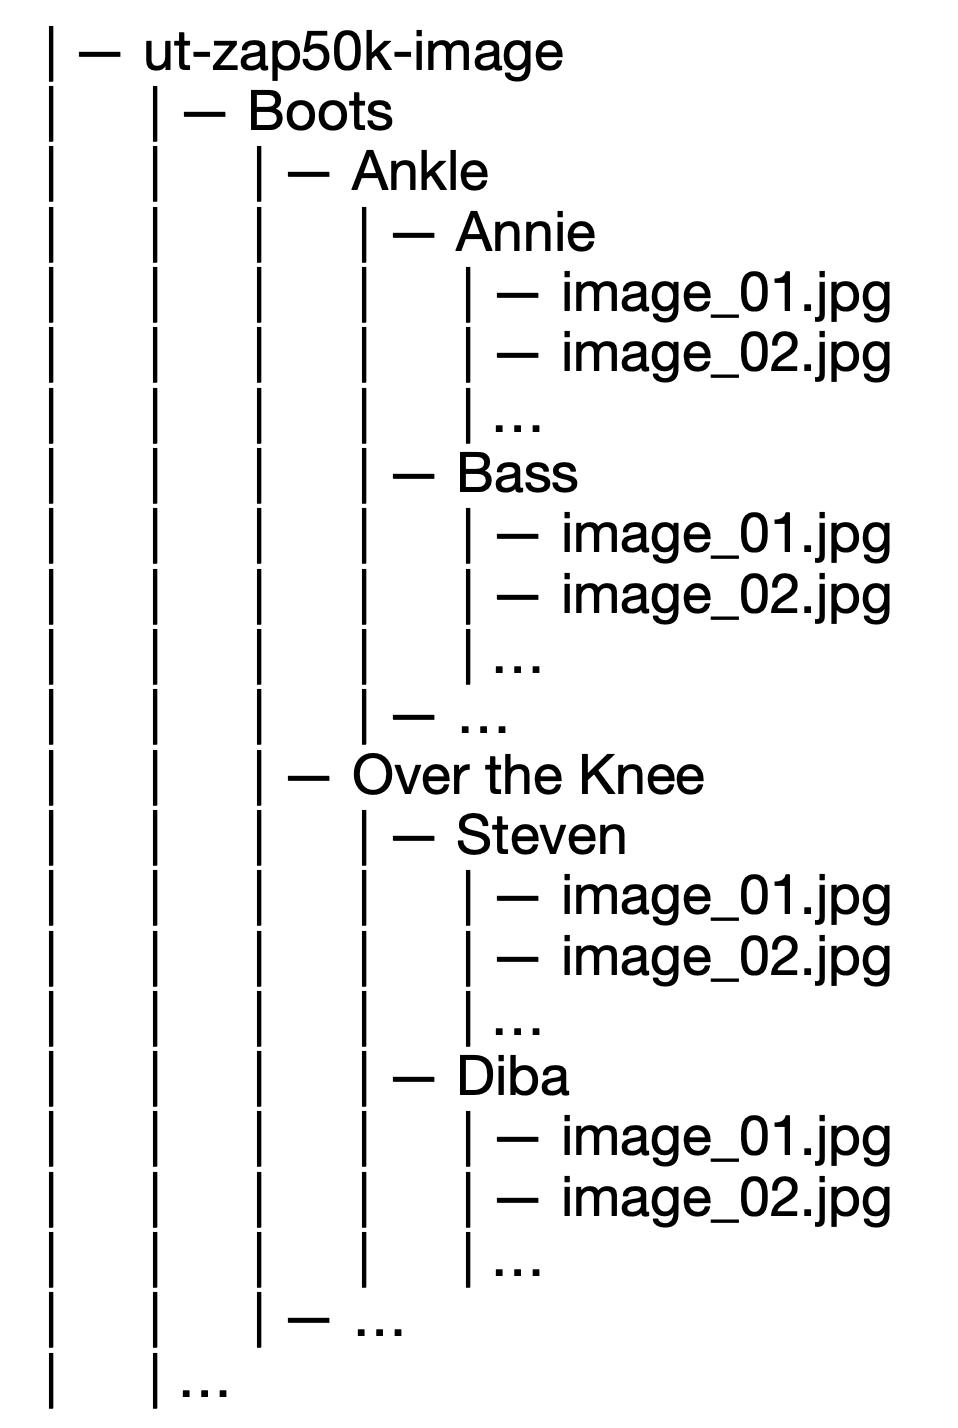
\includegraphics[width=0.5\linewidth]{figs/data_folder.png}
	\caption{An example of the folder structure of dataset }
	\label{fig:data_folder}
\end{figure}

\begin{figure}[h]
	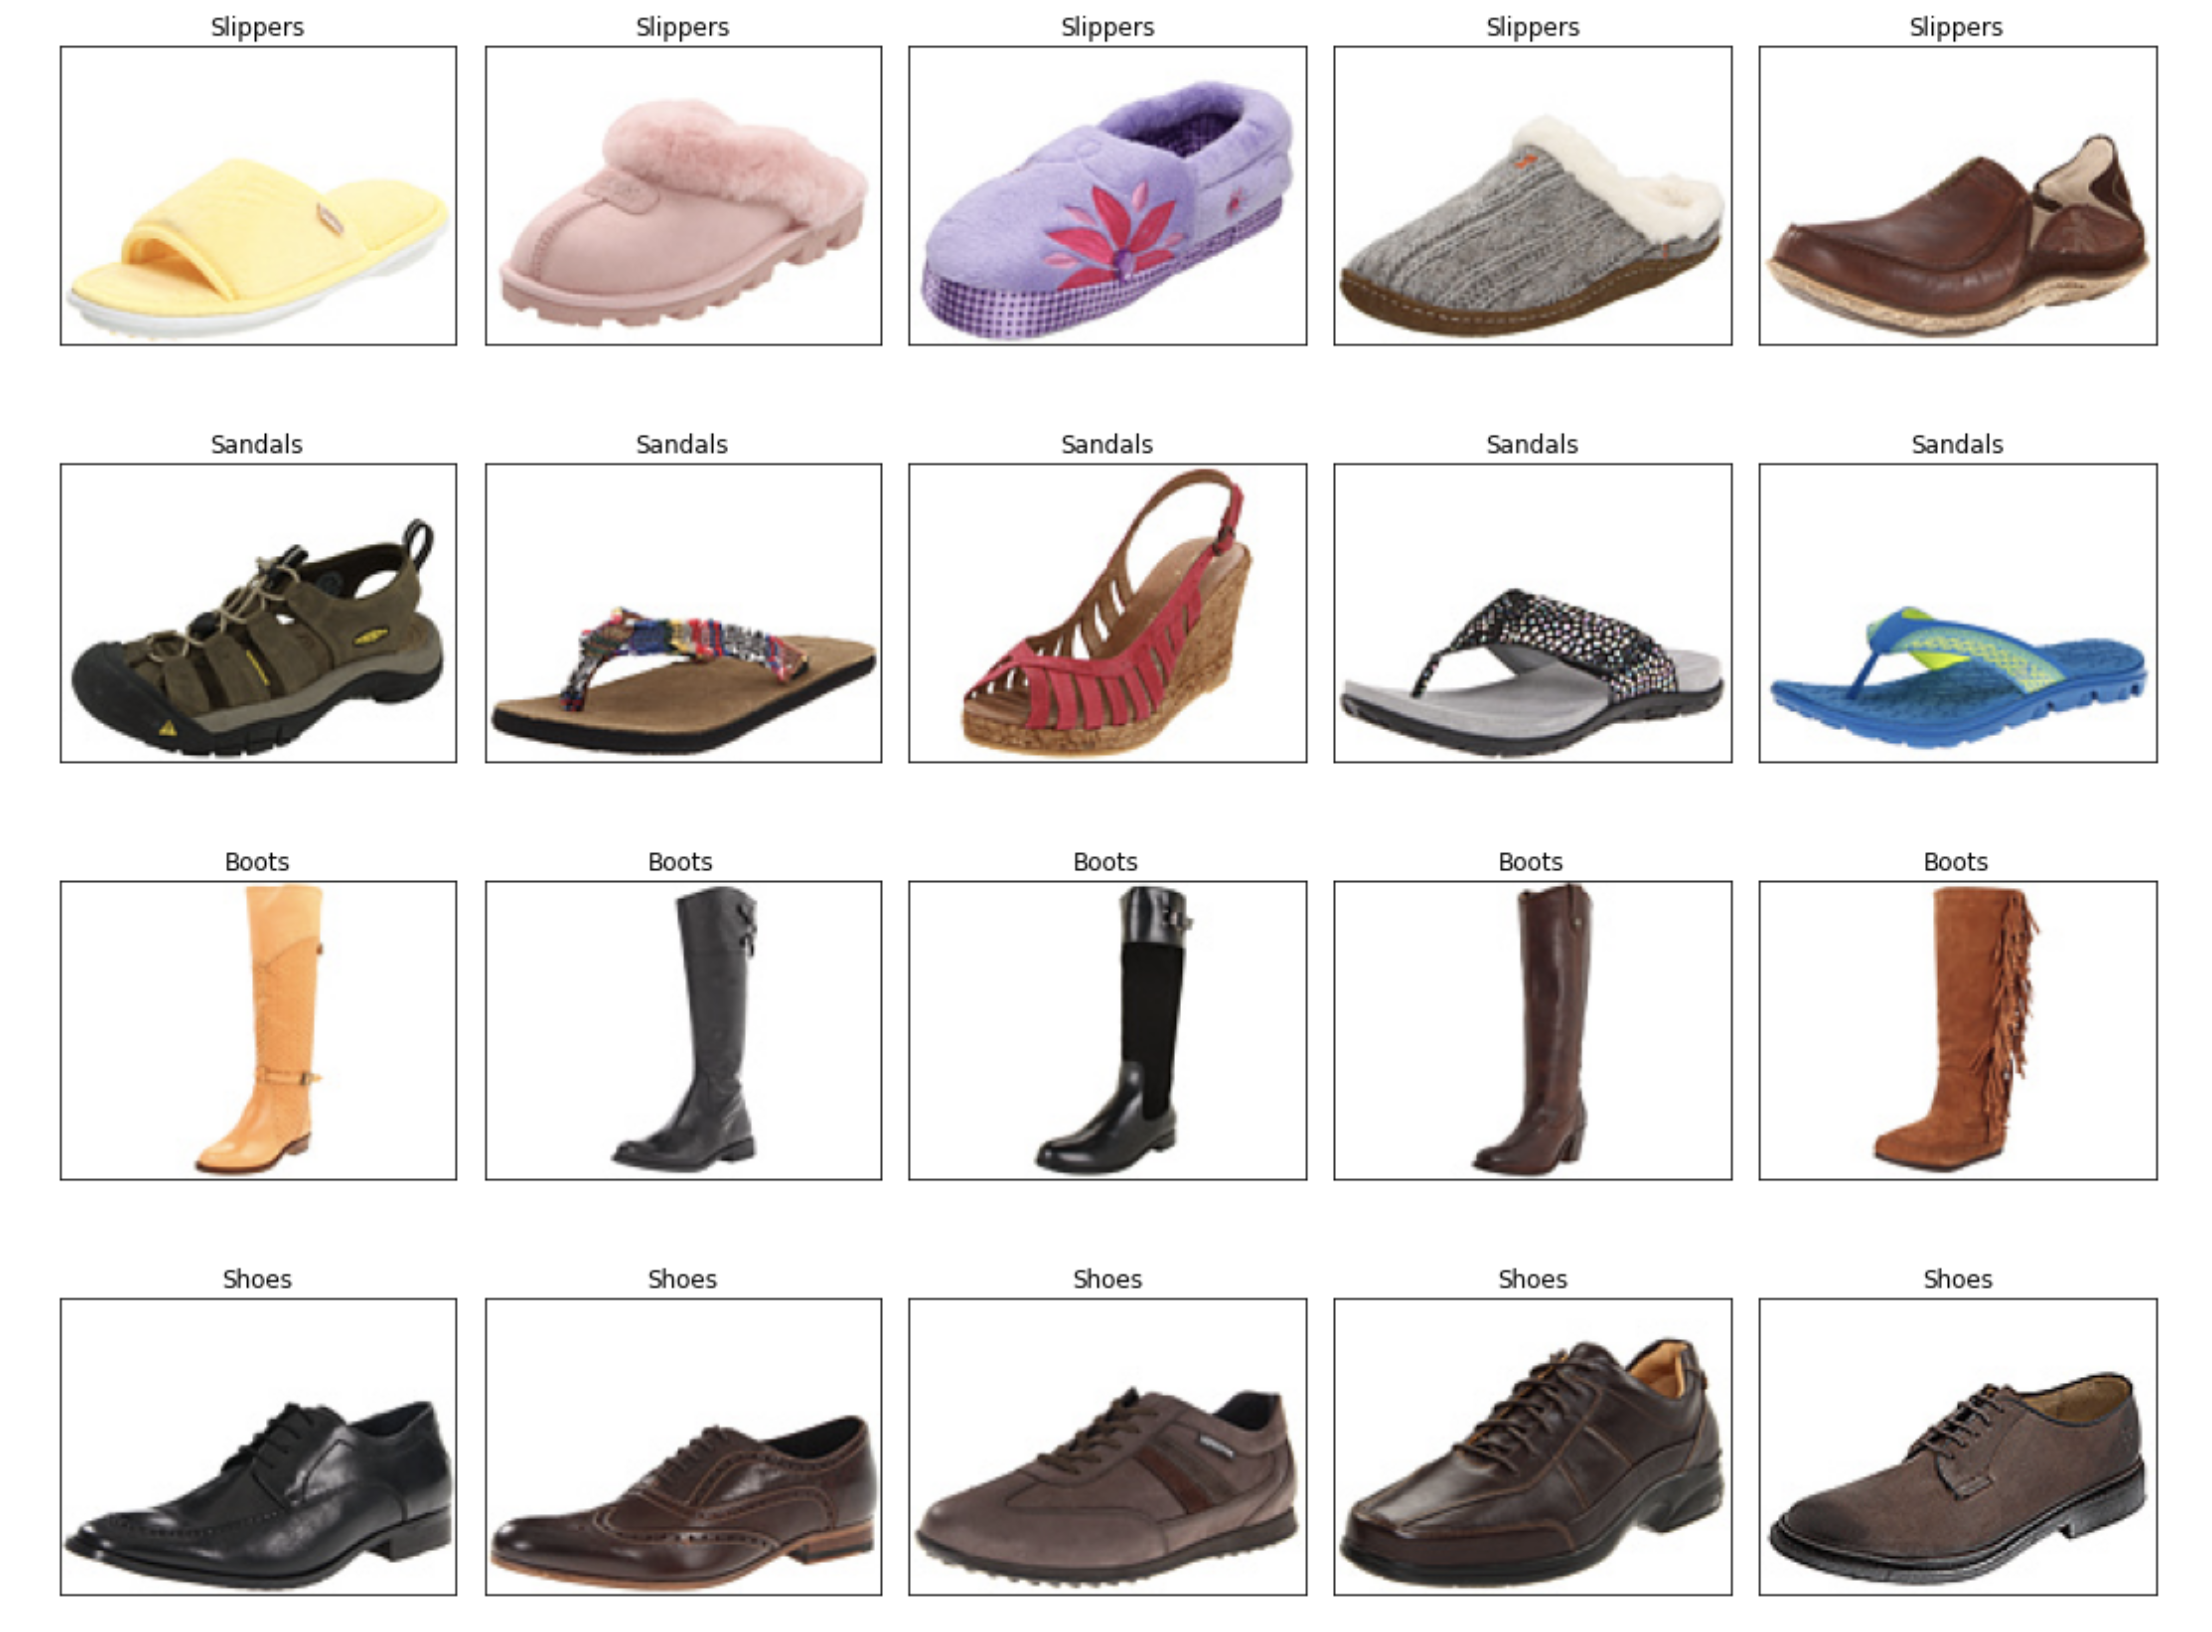
\includegraphics[width=\linewidth]{figs/data_example.png}
	\caption{An example of four categories in the dataset }
	\label{fig:data_example}
\end{figure}

\begin{table}[ht]
    \caption{Data distribution} 
    \centering 
    \begin{tabular}{c c c c} 
    \hline\hline 
    Shoes & Slippers & Sandals & Boots  \\% inserts table
    \hline % inserts single horizontal line
    30169 & 1283 & 5741 & 12832 \\% inserting body of the table
    1500 & 1283 & 1500 & 1500 \\% inserting body of the table
    2500 & 2500 & 2500 & 2500 \\% inserting body of the table
    \hline 
    \end{tabular}
\label{table:data} % is used to refer this table in the text
\end{table}

In this project, we only need the four major categories. So we merge all the images in each sub-folders, shown in figure \ref{fig:data_folder} into the category folder. In this way, we can label each image with its category folder name. Moreover, the first row of table \ref{table:data} represents the distribution of the four categories. We can see that the distribution of the dataset is very imbalanced. Especially, slippers are fewer than others. To create a balanced dataset for better accuracy calculation, we choose the first 1500 images from each category except Slippers, which use all the images. So in total, we have 5783 samples, as shown in the second row of table \ref{table:data}.

Besides, we know data argumentation such as flips, translations or rotations is good for getting more images. The ImageOps module contains some image processing operations. So we choose the mirror function, actually, it is the same as horizontal flip. In this way, we try to create a larger sub-dataset, which is shown in the third row of table, \ref{table:data} for the slippers class. In this project, we conduct an experiment to study the impact on augmenting a single class of the dataset.

On the other hand, our models implemented in this project all work well with a small dataset. Then we partition these samples into train, test, validation datasets with a ratio of 8:1:1. 

